\documentclass[tikz, border=5mm]{standalone}
\usepackage{textcomp}
\usetikzlibrary{arrows.meta,decorations.markings,fit,calc, positioning}

\definecolor{componentColor}{RGB}{210,210,210}
\definecolor{systemColor}{RGB}{230,230,230}

\tikzset{component/.append style={fill=componentColor, align=center, draw, minimum width=2cm, minimum height=1.5cm, rounded corners=.3cm,node distance=2cm and 1.5cm}}
\tikzset{system/.style={component, fill=systemColor, rounded corners=0cm}}
\tikzset{interface/.style={system, fill=systemColor, minimum size=1.6cm}}


\begin{document}

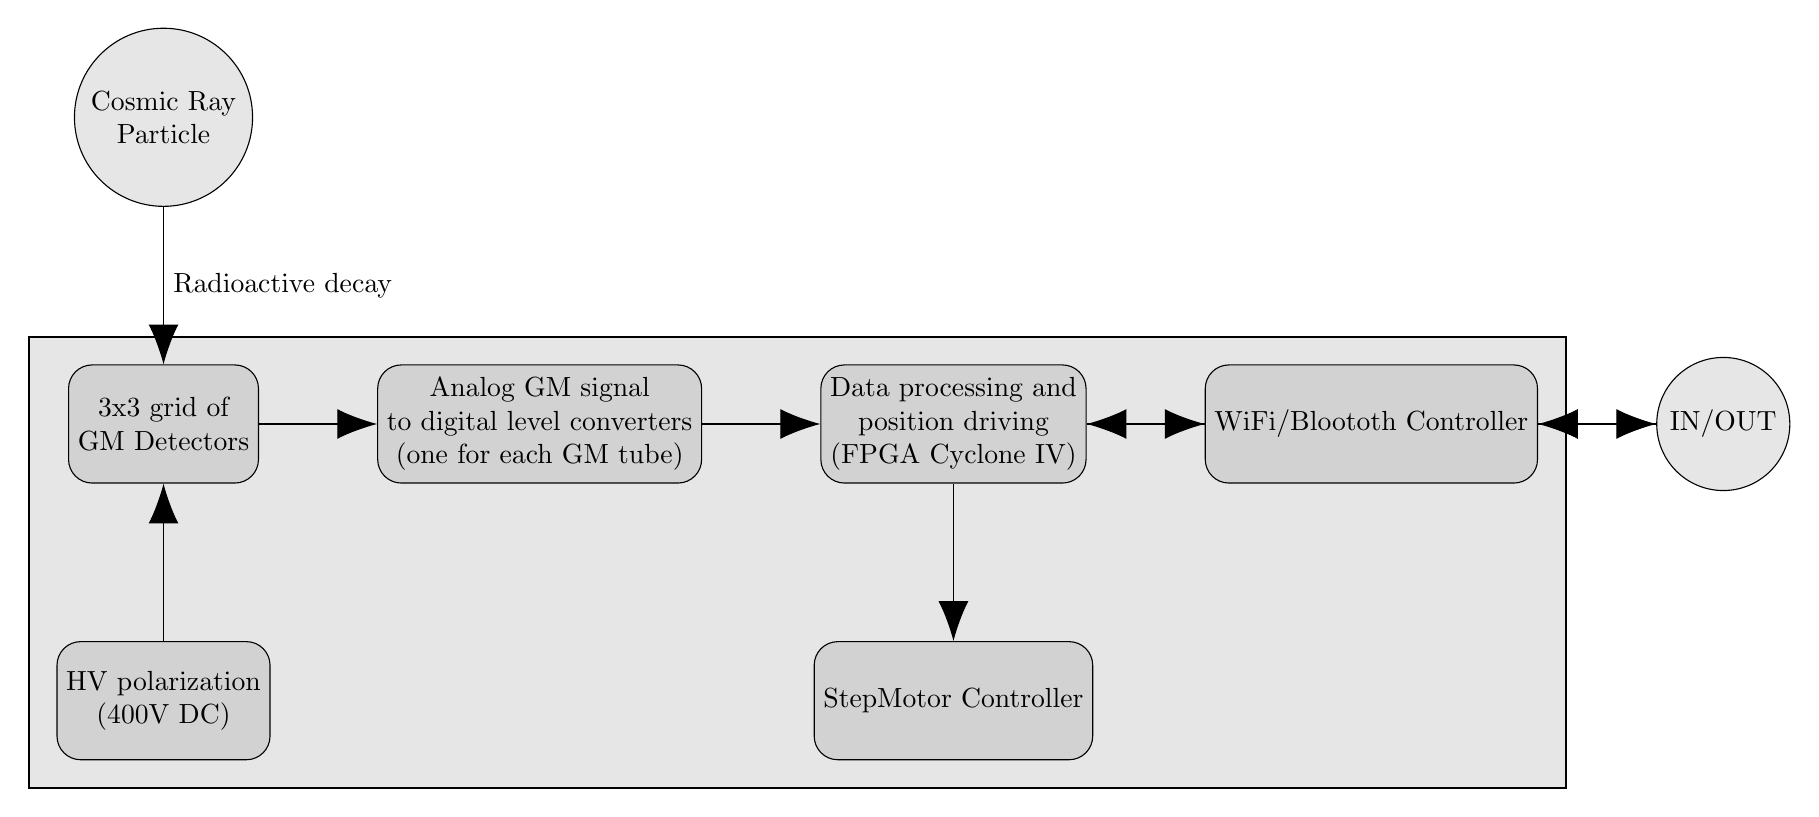
\begin{tikzpicture}[node distance=1.5cm and 3cm]
% Nodes
\pgfdeclarelayer{background}
\pgfsetlayers{background,main}

\node (CosmicRayParticle) [circle, interface] {Cosmic Ray\\ Particle};

\node (GMTubes) [component, below=of CosmicRayParticle] {3x3 grid of\\ GM Detectors};

\node (PolarizationVoltage) [component, below=of GMTubes] {HV polarization\\ (400V DC)};

\node (GMDataPreProcessing) [component, right=of GMTubes] {Analog GM signal\\ to digital level converters \\ (one for each GM tube)};

\node (GMDataProcessing) [component, right=of GMDataPreProcessing] {Data processing and\\ position driving\\ (FPGA Cyclone IV)};

\node (StepMotorController) [component, below=of GMDataProcessing] {StepMotor Controller};

\node (WiFiBlootothController) [component, right=of GMDataProcessing] {WiFi/Bloototh Controller};

\node (OutputInterface) [circle, interface, right=of WiFiBlootothController] {IN/OUT};


\begin{pgfonlayer}{background}
\node[system, draw, thick, inner xsep=1em, inner ysep=1em, fit= (PolarizationVoltage) (GMDataPreProcessing) (GMDataProcessing) (StepMotorController) (WiFiBlootothController)] {};
\end{pgfonlayer}

% Connectors
\begin{scope}[->]

\draw [-{Latex[scale=3.0]}] (CosmicRayParticle) -- node[anchor=west, minimum width=.25cm, draw=none] {Radioactive decay} (GMTubes);

\draw [-{Latex[scale=3.0]}] (GMTubes) -- node[anchor=west, minimum width=.25cm, draw=none] {} (GMDataPreProcessing);
\draw [-{Latex[scale=3.0]}] (PolarizationVoltage) -- node[anchor=west, minimum width=.25cm, draw=none] {} (GMTubes);
\draw [-{Latex[scale=3.0]}] (GMDataPreProcessing) -- node[anchor=west, minimum width=.25cm, draw=none] {} (GMDataProcessing);

\draw [-{Latex[scale=3.0]}] (GMDataProcessing) -- node[anchor=west, minimum width=.25cm, draw=none] {} (WiFiBlootothController);
\draw [-{Latex[scale=3.0]}] (WiFiBlootothController) -- node[anchor=west, minimum width=.25cm, draw=none] {} (GMDataProcessing);

\draw [-{Latex[scale=3.0]}] (GMDataProcessing) -- node[anchor=west, minimum width=.25cm, draw=none] {} (StepMotorController);

\draw [-{Latex[scale=3.0]}] (WiFiBlootothController) -- node[anchor=west, minimum width=.25cm, draw=none] {} (OutputInterface);
\draw [-{Latex[scale=3.0]}] (OutputInterface) -- node[anchor=west, minimum width=.25cm, draw=none] {} (WiFiBlootothController);



\end{scope}

\end{tikzpicture}
\end{document}
